\section{基本采样算法}
本节中,我们研究从一个给定的概率分布中生成随机样本的一些简单的方法。
\subsection*{标准概率分布}
首先,我们考虑如何从简单的非均匀分布中生成随机数,假定我们已经有了一个均匀分布的随机数的来源。假设$z$在区间$(0,1)$上均匀分布,我们使用某个函数$f(\cdot)$对$z$的值进行变换,即$y=f(z)$。$y$上的概率分布为
\begin{equation}
\label{suiji}
	p(y)=p(z)\bigg|\frac{\mathrm{d}z}{\mathrm{d}y}\bigg|
\end{equation}
其中,在这种情况下,$p(z)=1$。我们的目标是选择一个函数$f(z)$使得产生出的$y$值具有某种所需的具体的分布形式$p(y)$,对公式$\ref{suiji}$进行积分,我们有
\begin{equation}
	z=h(y)\equiv \int _{-\infty}^{y}p(\hat{y})d\hat{y}
\end{equation}
它是$p(y)$的不定积分,因此$y=h^{-1}(z)$,因此我们必须使用一个函数来对这个均匀分布的随机数进行变换,这个函数是所求的概率分布的不定积分的反函数,如图所示
\begin{center}
	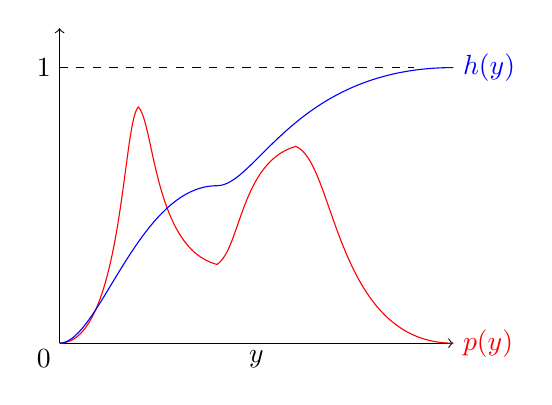
\begin{tikzpicture}
		\draw[->] (0,0) -- (5,0) node at (-0.2,3.5) {$1$};
		\draw[->] (0,0) -- (0,4) node at (-0.2,-0.2){$0$};
		\draw[dashed] (0,3.5) -- (4.5,3.5) node at (2.5,-0.2) {$y$};
		
		\draw[red]  
		(0,0) .. controls (0.8,0) and (0.8,2.8)  ..  (1,3) .. controls (1.2,2.8) and (1.2,1.2) .. (2,1) .. controls (2.3,1.2) and (2.3,2.3) .. (3,2.5) .. controls (3.5,2.3) and (3.5,0) .. (5,0) node[right] {$p(y)$};
		\draw[blue] (0,0) .. controls (0.5,0) and (1,2) .. (2,2) .. controls (2.5,2) and (3,3.5) ..(5,3.5) node[right] {$h(y)$};

	\end{tikzpicture}
\end{center}

考虑指数分布(exponential distribution)
\begin{equation}
	p(y)=\lambda \exp (-\lambda y)
\end{equation}
其中$0\leqslant y \leqslant \infty$。在这种情况下
\begin{equation}
	h(y)=\int_0^y f(y)dy=1-\exp (-\lambda y)
\end{equation}
从而,如果我们将均匀分布的变量$z$使用$y=-\lambda^{-1}\ln (1-z)$进行变换,那么$y$就会服从指数分布。
\begin{equation}
\begin{aligned}
	z&=h(y)=1-\exp (-\lambda y)\\
	y&=h^{-1}(z)\\
	 &\Rightarrow \exp(-\lambda y) = 1-z\\
	 &\Rightarrow -\lambda y = \ln (1-z)\\
	 &\Rightarrow y=-\frac{1}{\lambda}\ln (1-z)
\end{aligned}
\end{equation}

另一种可以应用变换方法的概率分布是柯西分布
\begin{equation}
	p(y)=\frac{1}{\pi}\frac{1}{1+y^2}
\end{equation}
这种情况下,不定积分的反函数可以用$\tan$函数表示。

对于多个变量情形的推广是很容易的,涉及到变量变化的Jacobian行列式,即
\begin{equation}
	p(y_1,\dots,y_M)=p(z_1,\dots,z_M)\bigg| \frac{\partial (z_1,\dots,z_M)}{\partial (y_1,\dots,y_M)}\bigg| 
\end{equation}

作为变换方法的最后一个例子,我们考虑Box-Muller方法,用于生成高斯概率分布的样本。首先我们生成一对均匀分布的随机变量$z_1,z_2\in (-1,1)$,我们可以这样生成:对$(0,1)$上的均匀分布的变量使用$z\to 2z -1$的方式进行变换。接下来,我们丢弃那些不满足$z_1^2+z_2^2\leqslant 1$的点对。这产生出单位圆内部的一个均匀分布,且$p(z_1,z_2)=\frac{1}{\pi}$。然后,对于每对$z_1,z_2$,我们计算 
\begin{flalign}
	y_1&=z_1\left(\frac{-2\ln r^2}{r^2} \right)^{\frac{1}{2}}\\
	y_2&=z_2\left(\frac{-2\ln r^2}{r^2} \right)^{\frac{1}{2}}
\end{flalign}
其中$r^2=z_1^2+z_2^2$。这样,$y_1$和$y_2$的联合概率分布为
\begin{equation}
	\begin{aligned}
		p(y_1,y_2)&=p(z_1,z_2)\bigg|\frac{\partial (z_1,z_2)}{\partial (y_1,y_2)} \bigg|\\
		&=\left[\frac{1}{\sqrt{2\pi}}\exp \left(\frac{-y_1^2}{2} \right) \right]\left[\frac{1}{\sqrt{2\pi}}\exp \left(\frac{-y_1^2}{2}\right) \right]
	\end{aligned}
\end{equation}
因此$y_1$和$y_2$是独立的,有每个都服从高斯分布,均值为零,方差为1。

\textbf{推导过程:}(Box-Muller变换原理)
\begin{enumerate}
	\item 目标
	\begin{equation}
	\begin{aligned}
		p(y_1,y_2)&=\left[\frac{1}{\sqrt{2\pi}}\exp \left(\frac{-y_1^2}{2} \right) \right]\left[\frac{1}{\sqrt{2\pi}}\exp \left(\frac{-y_1^2}{2}\right) \right]\\
		&=\frac{1}{2\pi}\exp \left(-\frac{y_1^2+y_2^2}{2} \right)
	\end{aligned}
	\end{equation}
	做极坐标变换,则$y_1=R\cos \theta,y_2=R\sin \theta$,则有
	\begin{equation}
		\frac{1}{2\pi}\exp \left(-\frac{y_1^2+y_2^2}{2} \right)=\frac{1}{2\pi}\exp \left(-\frac{R^2}{2} \right)
	\end{equation}
	可以看到这个结果可以看成是两个概率分布的密度函数的乘积,其中一个可以看成是$[0,2\pi]$上均匀分布,将其转换为标准均匀分布则有$\theta \sim U(0,2\pi)=2\pi z_1$,因为($z_1,z_2\sim U(0,1)$)。
	\item 求$h(y_1,y_2)$
	\begin{equation}
		\begin{aligned}
			z&=P(R\leqslant r)\\
			 &=\int_0^{2\pi} d\theta\int_0^r \frac{1}{2\pi}\exp \left(-\frac{\rho^2}{2} \right)\rho d\rho\\
			 &=-\exp\left(\frac{-\rho^2}{2}\right)\bigg|_0^r \\
			 &=-\exp \left(-\frac{r^2}{2}\right)+1
		\end{aligned}
	\end{equation}
	其中$r^2=z_1^2+z_2^2$。
	\item 求$y1,y2$
	\begin{equation}
		\begin{aligned}
			R&=h^{-1}(z)\\
			&=\sqrt{-2\ln (1-z)}
		\end{aligned}
	\end{equation}
	这里是二维联合分布,因此
	\begin{equation}
		\begin{aligned}
			y_1&=R\cos \theta = \frac{z_1}{r} \sqrt{-2\ln (r^2)}\\
			y_2&=R\sin \theta = \frac{z_2}{r} \sqrt{-2\ln (r^2)}
		\end{aligned}
	\end{equation}
\end{enumerate}

显然,变换方法依赖于它能够进行计算所需的概率分布,并且能够求所需的概率分布的不定积分的反函数。这样的计算只对于一些非常有限的简单的概率分布可行,因此我们必须寻找一些更加一般的方法。这里,我们考虑两种方法,即拒绝采样(rejection sampling)和重要采样(importance sampling)。虽然这些方法主要限制在单变量概率分布,因此无法直接应用于多维的复杂问题,但是这些方法确定是更一般的方法的重要成分。
\subsection*{拒绝采样}
拒绝采样框架使得我们能够在满足某些限制条件的情况下,从相对复杂的概率分布中采样。首先,我们考虑单变量分布,然后接下来讨论对于多维情形的推广。

假设我们希望从$p(\boldsymbol{z})$中采样,这个概率分布不是我们目前为止讨论过的简单的标准的概率分布中的一个,从而直接从$p(\boldsymbol{z})$中采样是很困难的。此外,我们假设我们能够很容易地计算对于任意给定的$\boldsymbol{z}$值的$p(\boldsymbol{z})$(不考虑归一化常数$Z$),即
\begin{equation}
	p(z)=\frac{1}{Z_p}\tilde{p}(z)
\end{equation}
其中$\tilde{p}(z)$可以很容易地计算,但是$Z_p$未知。

为了应用拒绝采样方法,我们需要一些简单的概率分布$q(z)$,有时被称为提议分布(proposal distribution),并且我们已经可以从提议分布中进行采样。接下来,我们引入一个常数k,它的值的选择满足下面的性质:对所有的z值,都有$kq(z)\geqslant \tilde{p}(z)$。函数$kq(z)$被称为比较函数。

拒绝采样器的每个步骤涉及到生成两个随机数。首先,我们从概率分布$q(z)$中生成一个数$z_0$。接下来,我们在区间$[0,kq(z)]$上的均匀分布中生成一个数$u_0$。这对随机数在函数$kq(z)$的曲线下方是均匀分布。最后,如果$u_0>\tilde{p}(z_0)$,那么样本被拒绝,否则$u_0$被保留。因此对应的$z$值服从概率分布$p(z)$,正如我们所需的那样。
\begin{center}
	\begin{tikzpicture}
		\filldraw[gray!50,line width=2] (-3,1) .. controls (-1,1) and (0,4).. (1,4) .. controls (2,4) and (3,1).. (5,1);
		\draw[pattern=north west lines,gray!50] (-3,0.1) rectangle (5,1);
		
		\filldraw[line width=2,draw=red,white] (-1.5,0.1) .. controls (-1,0.1) and (-0.7,2).. (0,2) .. controls (0.3,2) and (0.7,1).. (1,1).. controls (1.3,1) and (1.5,3).. (2,3) .. controls (2.5,3) and (2.5,0.1).. (4,0.1);
		
		\draw[->] (-3,0) -- (5,0) node[below] at (0,0){$z_0$};
		\draw[->] (0,0) -- (0,4);
		
		\node[fill,draw,circle,inner sep=0.5mm,black,label=left:$u_0$] at (0,1) {};
		\node[fill,draw,circle,inner sep=0.5mm,black,label=left:$kq(z_0)$] at (0,3.3) {};
		\node[label=left:$\tilde{p}(z)$] at (3,1) {};
		\node[black,label=left:$kq(z)$] at (3,4) {};
	\end{tikzpicture}
\end{center}
$z$的原始值从概率分布$q(z)$中生成,这些样本之后被接受的概率为$\frac{\tilde{p}(z)}{kq(z)}$,因此一个样本会被接受的概率为
\begin{equation}
	\begin{aligned}
		p(\text{接受})&=\int \left\{\frac{\tilde{p}(z)}{kq(z)} \right\}q(z)dz\\
		&=\frac{1}{k}\int \tilde{p}(z)dz
	\end{aligned}
\end{equation}
因此,被这种方法拒绝的点的比例依赖于曲线$kq(z)$下方的未归一化概率分布$\tilde{p}(z)$的面积的比例。于是,我们看到,常数k应该尽量小,同时满足下面的限制条件:$kq(z)$一定处处不小于$\tilde{p}(z)$。
\subsection*{可调节的拒绝采样}
在许多我们希望应用拒绝采样的情形中,确定概率分布$q(z)$的一个合适的解析形式是很困难的。另一种确定其函数形式的方法是基于概率分布$p(z)$的值直接构建函数形式。

对于$p(z)$是对数凹函数的情形,即$\ln p(z)$的导数是$z$的单调非增函数时,界限函数的构建是相当简单的。函数$\ln p(z)$和它的切线在某些初始的格点处进行计算,生成的切线的交点被用于构建界限函数。接下来,我们从界限分布中抽取一个样本值。因为界限函数的对数是一系列的线性函数,因此界限函数本身由一个分段指数分布组成,形式为
\begin{equation}
	q(z)=k_i\lambda_i\exp \{-\lambda_i(z-z_i) \}\quad \hat{z}_{i-1,i}<z\leqslant \hat{z}_{i,i+1}
\end{equation}
其中$\hat{z}_{i-1,i}$是在点$z_{i-1}$和$z_i$处的切线的交点,$\lambda_i$是切线在$z_i$处的斜率,$k_i$表示对应的偏移量。一旦一个样本点被抽取完毕,我们就可以应用通常的拒绝准则了。如果样本被接受,那么它就是所求的概率分布中的一个样本。然而,如果样本被拒绝,那么它被并入的集合中,计算出一条新的切线,从而界限函数被优化。随着格点数量的增加,界限函数对所求的概率分布的近似效果逐渐变好,拒绝的概率就会减小。

这个算法存在一种变体,这种变体中不用计算导数。可调节的拒绝采样的框架也可以扩展到不是对数凹函数的概率分布中,只需将每个拒绝采样的步骤中使用Metropolis-Hasting阶梯函数即可,这就产生了可调节拒绝Metropolis采样(adaptive rejection Metropolis sampling)方法。

显然,对于具有实际价值的拒绝采样来说,我们要求对比函数要接近所求的概率分布,从而拒绝率要保持一个最小值。对于更实际的例子来说,所求的概率分布可能是多峰的,并且具有尖峰,从而找到一个较好的提议分布和比较函数是一件相当困难的事情。此外,接受率随着维度的指数下降是拒绝采样的一个一般特征。虽然拒绝采样在一维或二维空间中是一个有用的方法,但是它不适用于高维空间。然而,对于高维空间中的更加复杂的算法来说,它起着子过程的作用。
\subsection*{重要采样}
想从复杂概率分布中采样的一个主要原因是能够使用公式$\ref{zhongyao}$计算期望。重要采样(importance sampling)的方法提供了直接近似期望的框架,但是它本身并没有提供从概率分布$p(z)$中采样的方法。

公式$\ref{youxian}$给出的期望的有限和近似依赖于能够从概率分布$p(z)$中采样。然而直接从$p(z)$中采样无法完成,但是对于任意给定的$z$值,我们可以很容易地计算$p(z)$。一种简单的计算期望的方法是将$z$空间离散化为均匀的格点,将被积函数使用求和的方式计算,形式为
\begin{equation}
	\mathbb{E}[f]\simeq \sum_{l=1}^{L}p(z^{(l)})f(z^{(l)})
\end{equation}
这种方法的一个明显的问题是求和式中的项的数量随着$z$的维度指数增长。此外,我们感兴趣的概率分布通常将它们的大部分质量限制在$z$空间的一个很小的区域,因此均匀地采样非常低效,因为在高维的问题中,只有非常小的一部分样本会对求和式产生巨大的贡献。我们希望从$p(z)$的值较大的区域中采样,或者理想情况下,从$p(z)f(z)$的值较大的区域中采样。

与拒绝采样的情形相同,重要采样基于的是对提议分布$q(z)$的使用,我们很容易从提议分布中采样。之后,我们可以通过$q(z)$中的样本$\{z^{(l)} \}$的有限和的形式来表示期望
\begin{equation}
	\begin{aligned}
		\mathbb{E}[f]&=\int f(z)p(z)dz\\
		&=\int f(z) \frac{p(z)}{q(z)}q(z)dz\\
		&\simeq \frac{1}{L}\sum_{l=1}^{L}\frac{p(z^{(l)})}{q(z^{(l)})}f(z^{(l)})
	\end{aligned}
\end{equation}
$r_l=\frac{p(z^{(l)})}{q(z^{(l)})}$被称为重要性权重(importance weights),修正了由于从错误的概率分布中采样引入的偏差。注意,与拒绝采样不同,所有生成的样本都被保留。

常见的情形是,概率分布$p(z)$的计算结果没有归一化,即$p(z)=\frac{\tilde{p}(z)}{Z_p}$,其中$\tilde{p}(z)$可以很容易地计算出来,而$Z_p$未知。类似地,我们可能希望使用重要采样分布$q(z)=\frac{\tilde{q}(z)}{Z_q}$,它具有相同的性质。于是我们有
\begin{equation}
	\begin{aligned}
		\mathbb{E}[f]&=\int f(z)p(z)dz\\
		&=\frac{Z_q}{Z_p}\int f(z)\frac{\tilde{p}(z)}{\tilde{q}(z)}q(z)dz\\
		&\simeq \frac{Z_q}{Z_p}\frac{1}{L}\sum_{l=1}^{L}\tilde{r}_l f(z^{(l)})
	\end{aligned}
\end{equation}
其中$\tilde{r}_l=\frac{\tilde{p}(z)}{\tilde{q}(z)}$。我们可以使用同样的样本集合来计算比值$\frac{Z_p}{Z_q}$,结果为
\begin{equation}
	\begin{aligned}
		\frac{Z_p}{Z_q}&=\int \frac{\tilde{p}(z)}{\tilde{q}(z)}q(z)dz\\
		&\simeq \frac{1}{L}\sum_{l=1}^{L}\tilde{r}_l
	\end{aligned}
\end{equation}
因此
\begin{equation}
	\mathbb{E}[f]\simeq \sum_{l=1}^{L}w_lf(z^{(l)})
\end{equation}
其中我们定义
\begin{equation}
	w_l=\frac{\tilde{r}_l}{\sum_m \tilde{r}_m}
\end{equation}
与拒绝采样的情形相同中,重要采样方法的成功严重依赖于采样分布$q(z)$与所求的概率分布$p(z)$的匹配程度。经常出现的情形是$p(z)$变化剧烈,并且大部分的质量集中于$z$空间的一个相对较小的区域中,此时重要权重$\{r_l\}$由几个具有圈套值的权值控制,剩余的权值相对较小。因此,有效的样本集大小会比表面上的样本集大小L小得多。如果没有样本落在$p(z)f(z)$圈套的区域中,那么问题会更加严重。此时,$r_l$和$r_lf(z^{(l)})$的表面上的方差可能很小,即使期望的估计可能错得离谱。因此,重要性采样方法的一个主要的缺点是它具有产生任意错误的结果的可能性,并且这种错误无法检测。这也强调 采样分布$q(z)$的一个关键的要求,即它不应该在$p(z)$可能圈套的区域中取得较小的值或者为零的值。
\subsection*{采样-重要性-重采样}
拒绝采样方法部分依赖于确定常数k的一个合适的值。对于许多对概率分布$p(z)$和$q(z)$来说,确定一个合适的k值是不现实的,因为任意的足够大的k值才能够保证产生所求的分布的上界,但是这会产生相当小的接受率。

与拒绝采样的情形相同,采样-重要性-重采样(sampling-importance-resampling,SIR)方法也使用采样$q(z)$,但是避免了必须确定常数$k$。这个方法有两个阶段,在第一个阶段,L个样本$z^{(1)},\dots,z^{(L)}$从$q(z)$中抽取。然后在第二个阶段,构建权值$w_1,\dots,w_L$。最后,L个样本的第二个集合从离散概率分布$(z^{(1)},\dots,z^{(L)})$中抽取,概率由权值$(w_1,\dots,w_L)$给定。
\subsection*{采样与EM算法}
蒙特卡罗方法除了为贝叶斯框架的直接实现提供了原理,还在频率学家的框架内起着重要的作用,例如寻找最大似然解。特别地,对于EM算法中的E步骤无法解析地计算的模型,采样方法也可以用来近似E步骤。

考虑一个模型,它的隐含变量为$Z$,可见(观测)变量为$X$,参数为$\theta$。在M步骤中关于$\theta$最大化的步骤为完整数据对数似然的期望,形式为
\begin{equation}
	Q(\theta,\theta^{\text{旧}})=\int p(Z|X,\theta^{\text{旧}})\ln p(Z,X|\theta)dZ
\end{equation}
我们可以使用采样的方法来近似这个积分,方法是计算样本$\{Z^{(l)} \}$上的有限和,这些样本是从当前的对后验概率分布$p(Z|X,\theta^{\text{旧}})$的估计中抽取的,即
\begin{equation}
	Q(\theta,\theta^{\text{旧}})\simeq \frac{1}{L}\sum_{l=1}^{L}\ln p(Z^{(l)},X|\theta)
\end{equation}
然后,Q函数在M步骤中使用通常的步骤进行优化。这个步骤被称为蒙特卡罗EM算法(Monte Carlo EM algorithm)。

现在假设我们从最大似然的方法转移到纯粹的贝叶斯方法,其中我们希望从参数向量$\theta$上的后验概率分布中进行采样。原则上,我们希望从联合后验分布$p(\boldsymbol{\theta},\boldsymbol{Z}|\boldsymbol{X})$中抽取样本,但是我们假设这个计算十分困难。进一步地,我们假设从完整数据参数的后验概率分布$p(\boldsymbol{\theta}|\boldsymbol{Z},\boldsymbol{X})$中进行采样相对简单。这就产生了数据增广算法(data augmentation algorithm),它在两个步骤之间交替进行,这两个步骤被称为I步骤(归咎(imputation)步骤,类似于E步骤)和P步骤(后验(posterior)步骤,类似于M步骤)。
\begin{enumerate}
	\item I步骤。我们希望从概率分布$p(\boldsymbol{Z}|\boldsymbol{X})$采样,但是我们不能直接进行。于是,我们注意到下面的关系
	\begin{equation}
		p(\boldsymbol{Z}|\boldsymbol{X})=\int p(\boldsymbol{Z}|\boldsymbol{\theta},\boldsymbol{X})p(\boldsymbol{\theta}|\boldsymbol{X})d\boldsymbol{X}
	\end{equation}
	因此对于$l=1,\dots,L$,我们首先从当前对$p(\boldsymbol{\theta}|\boldsymbol{X})$的估计中抽取样本$\boldsymbol{\theta}^{(l)}$,然后使用这个样本从$p(\boldsymbol{Z}|\boldsymbol{\theta}^{(l)},\boldsymbol{X})$中抽取样本$\boldsymbol{Z}^{(l)}$。
	\item P步骤。给定关系
	\begin{equation}
		p(\boldsymbol{\theta}|\boldsymbol{X})=\int p(\boldsymbol{\theta}|\boldsymbol{Z},\boldsymbol{X})p(\boldsymbol{Z}|\boldsymbol{X})d\boldsymbol{Z}
	\end{equation}
	我们使用从I步骤中得到的样本$\{\boldsymbol{Z}^{(l)} \}$,计算$\boldsymbol{\theta}$上的后验概率分布的修正后的估计,结果为
	\begin{equation}
		p(\boldsymbol{\theta}|\boldsymbol{X})\simeq \frac{1}{L}\sum_{l=1}^{L}p(\boldsymbol{\theta}|\boldsymbol{Z}^{(l)},\boldsymbol{X})
	\end{equation}
	根据假设,在I步骤中从这个近似分布中采样是可行的。
\end{enumerate}

注意,我们对参数$\boldsymbol{\theta}$和隐含变量$\boldsymbol{Z}$进行了区分。从现在开始,我们不进行这种区分,仅仅集中于从给定的后验概率分布中抽取样本的问题。